%!TEX root = ../main.tex

\chapter{网格同坯近似算法}
在上一章中我们介绍了现有的四种比较主流的网格简化算法。就简化结果而言,相对复杂的基于内外壳的简化算法不仅能够更好地控制简化误差,而且能够在相同误差下获得更高的简化程度,在相同的简化程度下获得更低的误差。最近Manish Mandad等人将网格重建和带有内外壳的网格简化算法进行了有机地结合,提出了一种新型的鲁棒的网格同坯近似算法\cite{isotopic-appro}。与其他基于内外壳的网格简化算法不同,该算法以给定误差空间的内外边界上的采样点为输入,先重建再简化,因此,对原网格的要求更低——只要能通过原网格生成比较好的内外边界采样点如图\ref{fig:iso-appro-robust}。该算法通过空间四面体化,并通过这个四面体网格中线性差值维护一个空间中的误差函数$\epsilon(s)$,来控制简化结果与原模型之间的误差在用户给定的范围内。该算法大致可以分为以下步骤:
\begin{enumerate}[(1)]
  \item 细化,构建误差空间Ω的近似Γ;
  \item 简化误差空间Γ的边界;
  \item 镶嵌 0-等值点;
  \item 简化 0-等值面;
  \item 所有可能的简化。
\end{enumerate}
\begin{figure}[htbp]
    \centering
    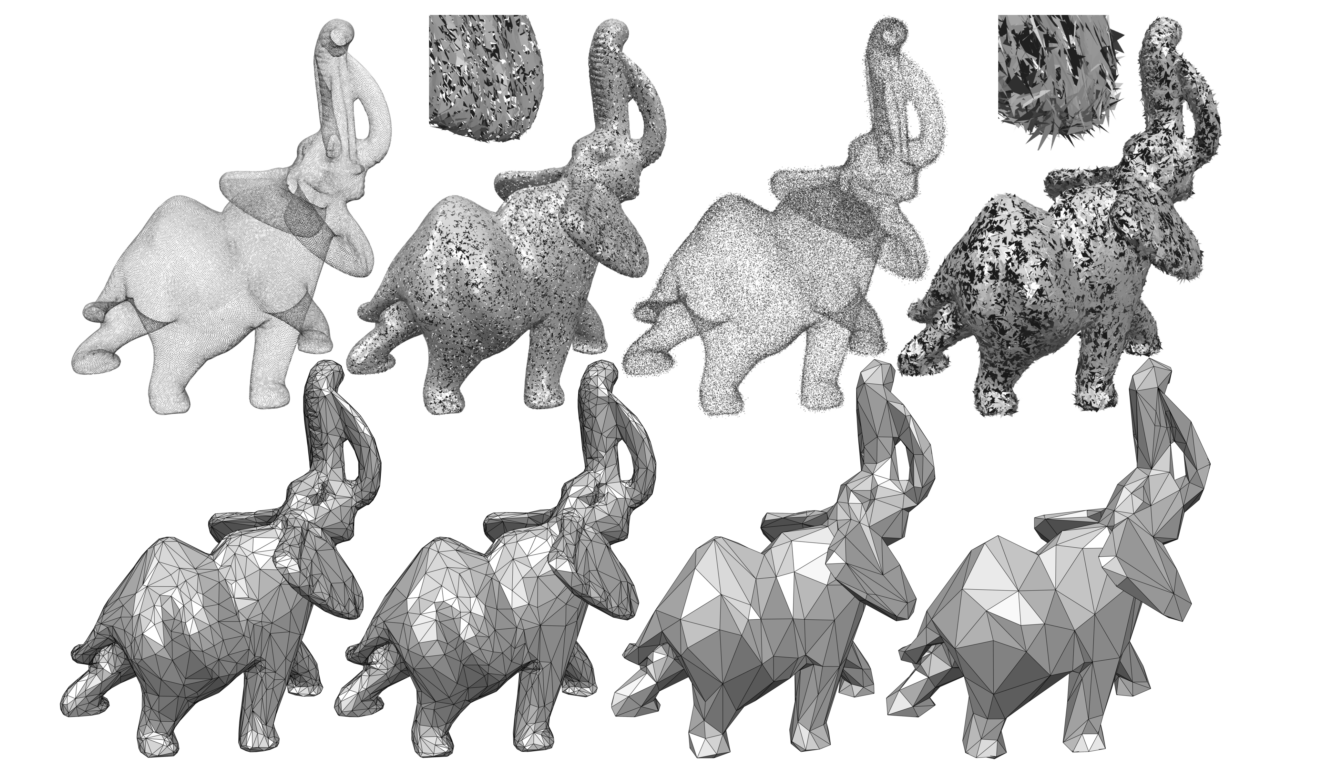
\includegraphics[width=.8\textwidth]{iso_appro_robust.png}
    \caption[同坯近似算法鲁棒性]{网格同坯近似算法能鲁棒地处理带有噪声的输入数据。从左到右分别是顶点集合,带有低噪声的三角面片集合,带有高噪声的顶点集合以及带有高噪声的三角面片集合。第二行是对这些数据的简化结果,图引用自\cite{isotopic-appro}}
    \label{fig:iso-appro-robust}
\end{figure}

\section{细化,构建误差空间Ω的近似Γ}
对于给定的误差空间为$\Omega$,算法以对误差空间$\Omega$的边界$\partial \Omega$上的一个密度为$\sigma$的采样(以每个采样点为圆心,以$\sigma$为半径的圆球,能够覆盖整个$\partial \Omega$)所得到的采样点集合S作为输入。算法假定这个误差空间只有两个边界,内边界和外边界,定义$S_0$为内边界采样点,$S_1$为外边界采样点,$S_{bs}$为包围球上的采样点。在S上定义一个参照函数:
\begin{equation}
  \begin{split}
    F(s) &= -1, s\in S_0\\
    F(s) &= +1, s\in S_1\\
    F(s) &= +1, s\in S_{bs}
  \end{split}
\end{equation}
然后以$\Omega$的包围球上的采样点$S_{bs}$作为初始化顶点,做一个四面体化,得到四面体网格$\tau$。在$\tau$上针对每一个四面体维护一个线性差值函数:
\begin{equation}
  f(s) = \sum_{i=0}^3 w_iF(s_i), s\in tet(s_0, s_1, s_2, s_3), s_i \in \tau
  \label{eq:linear-interpolation}
\end{equation}
这里,$tet(s_0, s_1, s_2, s_3)$是由这四个顶点所构成的四面体,$w_i$是顶点s在这个四面体上的重心坐标分量。所谓重心坐标是指对于四面体$tet(s_0, s_1, s_2, s_3)$中的一个顶点s,我们可以通过这四个点的加权来得到s的坐标值即:
\begin{equation}
  \begin{split}
  \sum_{i=0}^3 w_i s_i &= s\\
  \sum_{i=0}^3 w_i &= 1
  \end{split}
  \label{eq:err-constraint}
\end{equation}
这样,我们就可以得到每一个内外壳上的采样点的对应函数值,定义所有$f(s)=0$的点的集合为$\mathcal{Z}$即0-等值面,而当内外采样点的$f(s)$函数值与参照函数$F(s)$的函数值相差不超过1的时候,这个0-等值面$\mathcal{Z}$能够正确地将$S_0$和$S_1$的采样点区分开,也即0-等值面不会超越误差空间(如图\ref{fig:isotopic-classification})。因此,在采样点S上定义一个误差函数:
\begin{equation}
  \epsilon(s) = \lVert f(s)-F(s) \rVert
\end{equation}
从而误差约束条件转化为:
\begin{equation}
  \forall s \in S, \epsilon(s)<1
\end{equation}

\begin{figure}[htbp]
    \centering
    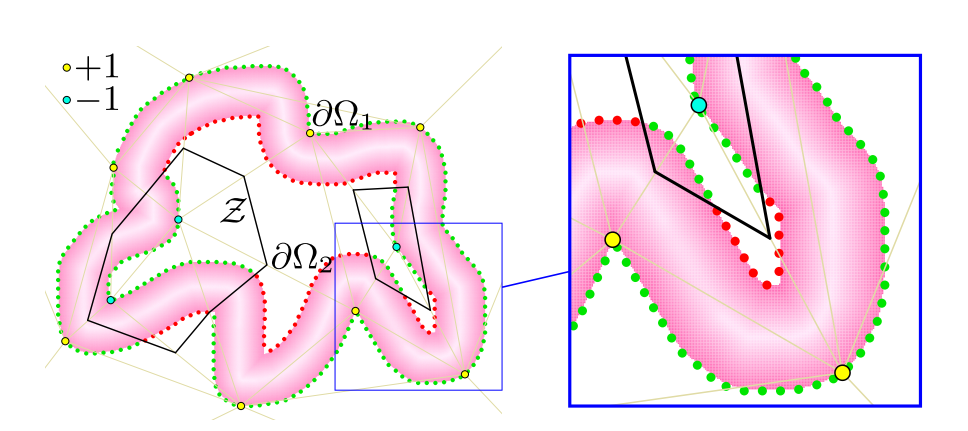
\includegraphics[width=.7\textwidth]{classification.png}
    \caption[0-等值面区分误差边界采样点]{图中绿色的点已经被0-等值面正确地分开,而红色的点未被正确地分开,图来自\cite{isotopic-appro}}
    \label{fig:isotopic-classification}
\end{figure}

\begin{figure}[htbp]
    \centering
    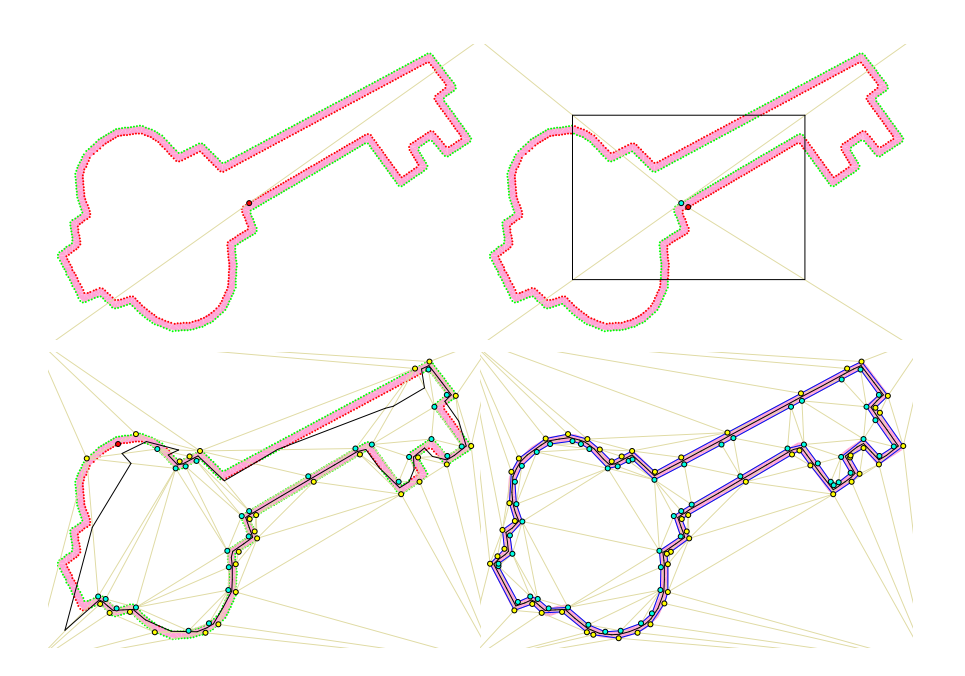
\includegraphics[width=.7\textwidth]{refine.png}
    \caption[细化过程]{细化的过程——逐渐地加入采样点直到所有的采样点能够被0-等值面正确地区分开,图来自\cite{isotopic-appro}}
    \label{fig:refine}
\end{figure}

\par 在细化阶段基本思路是:使用贪心的策略不断地选取$s \in S,\epsilon(s)$最大的顶点加入到$\tau$中,并重做四面体化直到直到$\tau$达到这个约束条件(如图\ref{fig:refine})。不过为了保持法向的质量,尽可能避免简化后的网格可能会出现法向翻转的问题(如图\ref{fig:normal-cond}),需要添加一个额外的法向约束条件:在每一个四面体上定义的线型差值函数不仅能够正确地区分在该四面体内的S中的采样点,而且当该四面体缩小到一个比例$\alpha$后,该线性差值函数也能够区分内外壳上离缩小的四面体的四个顶点最近的采样点。在整个细化的过程中,依次判断误差约束条件,以及法向约束条件是否得到满足。
\begin{figure}[htbp]
    \centering
    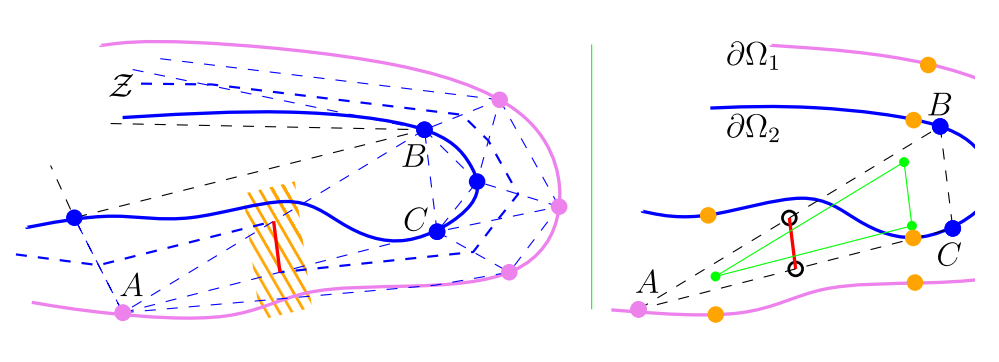
\includegraphics[width=.7\textwidth]{normal_cond.png}
    \caption[法向约束条件]{由于三角化不合理导致的法向不合理的情况(左图红色边)。右图是对法向是否合理的一个检测,红色的边并不能将绿色三角形($\triangle ABC$缩小一定比例之后的三角形)的三个顶点最近的内外壳采样点(橘黄色的顶点)正确地划分开,图来自\cite{isotopic-appro}}
    \label{fig:normal-cond}
\end{figure}
为了得到一个质量相对较好的四面体网格$\tau$(尽量避免细长的四面体出现),使用3D Delaunnay三角化来为空间中的顶点构建四面体网格。对于$\mathbb{R}^3$上的顶点集合S,其3D Delaunay三角化$(DT)$的结果$D(S)$是一个满足对于任意一个$D(S)$上的四面体,没有其他顶点落在它的外接球内部(如图\ref{fig:2d-delaunay})。对于$S$上的一个3D三角化$\tau$,对于一个三角面片$f \in \tau$,若$f$与由其所构成的四面体的任一外接球中的顶点均没有边相连,那么我们所这个三角面片f是局部Delaunay的。如果$\tau$中的所有三角面片都是局部Delaunay的,那么$\tau \equiv D(S)$。3D Delaunnay三角化的一个重要特点是能够最小化四面体网格中四面体的最大外接球。因此,3D Delaunay三角化能够尽可能避免一些狭长的四面体的出现,获得质量较好地四面体网格。在细化结束后,就得到了一个原误差空间$\Omega$的近似$\Gamma$。也得益于3D Delaunay三角化,对于不满足法向约束条件的四面体,可以选取离该四面体外接球球心最近的采样点加入到四面体网格$\tau$中,然后更新四面体网格$\tau$。由于采用3D Delaunay三角化的性质,加入这样的点会破坏原不满足法向约束条件的四面体(在新的题网格$\tau$中,这四个点不构成一个四面体),从而达到了消除不满足法向约束条件的四面体的功能。
\begin{figure}[htbp]
    \centering
    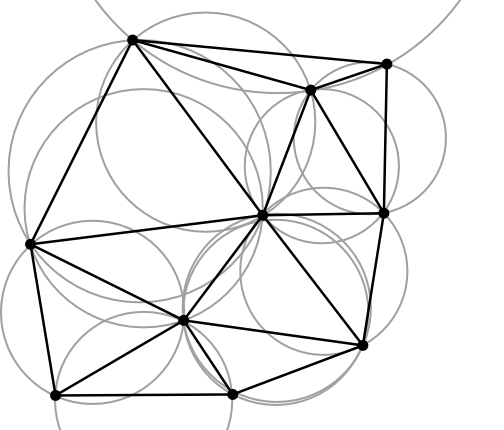
\includegraphics[width=.5\textwidth]{2d_delaunay.png}
    \caption[2D Delaunay]{2D上的Delaunnay三角化示意图,引用自\cite{delaunay-wiki}}
    \label{fig:2d-delaunay}
\end{figure}

\section{误差边界$\partial \Gamma$的简化}
在初始化得到了一个满足误差控制要求的四面体网格$\tau$,通过消除这个近似误差空间$\Gamma$的边界$\partial \Gamma$上的边来简化$\partial \Gamma$。首先需要保证简化过后的四面体网格$\tau$仍然是一个有效的四面体网格:
\begin{enumerate}[(1)]
  \item 四面体网格的拓扑结构是有效的(保证不会出现不属于任何四面体的面等);
  \item 四面体网格是包围球空间的一个有效的填充,即不存在相互交叉的四面体。
\end{enumerate}
为了保证简化后的τ足第一个条件,需要保证我们消除的边需满足Dey等人提出的Link Condition\cite{link-cond},而对于第二个条件需要使得消除的边的合并点落在这条边的Kernel Region中。除了上述两个基本的条件外,还需要保简化满足误差约束条件\eqref{eq:err-constraint},以及为了维持法向质量所加的法向约束。

\subsection{Link Condition}
借鉴Dey等人对保持拓扑有效性的消边的研究,在$\tau$上做消边操作时,需要判断该边是否满足Link Condition。一个由k+1个独立的点构成的凸包$\sigma$,被称为k-simplex,比如 0-simplex ——点,1-simplex ——线段。$\sigma$上的一个非空子集t,称为$\sigma$的face,而相对的$\sigma$是t的coface。定义由有限个k-simplex构成的一个集合$\mathcal{K}$,称为simplical complex。这里的四面体网格$\tau$就是这样的一个simplical complex。假设B是一个simplical complex $\mathcal{K}$上的一个子集,则定义B的closure ——$\overline{B}$(如图\ref{fig:closure}),为包含B中所有face的最小simplical complex。而B的star ——$St B$(如图\ref{fig:star}),定义为包含B中每一个simplex的star的并集,一个simpex的star即为该simplex的coface。而Lk(B):$Lk B = \overline{St B} - St \overline{B}$(如图\ref{fig:link})。\par

\begin{figure}[htbp]
    \centering
    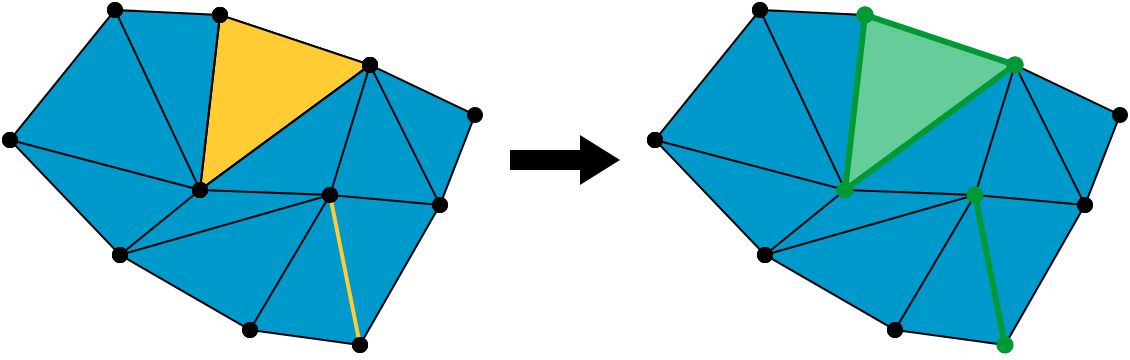
\includegraphics[width=.7\textwidth]{simplicial_complex_closure.png}
    \caption[2D closure]{2D三角网格上的closure示意图,图引用自\cite{simplicial-complex}}
    \label{fig:closure}
\end{figure}
\begin{figure}[htbp]
    \centering
    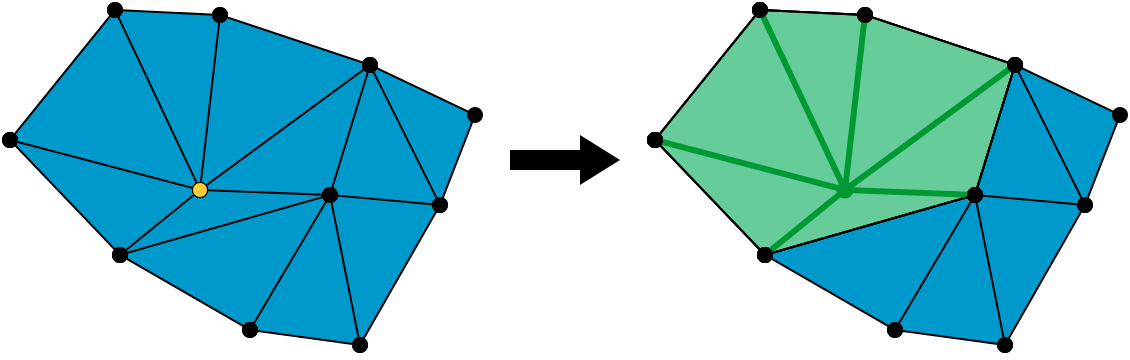
\includegraphics[width=.7\textwidth]{simplicial_complex_star.png}
    \caption[2D star]{2D三角网格上的star示意图,图引用自\cite{simplicial-complex}}
    \label{fig:star}
\end{figure}
\begin{figure}[htbp]
    \centering
    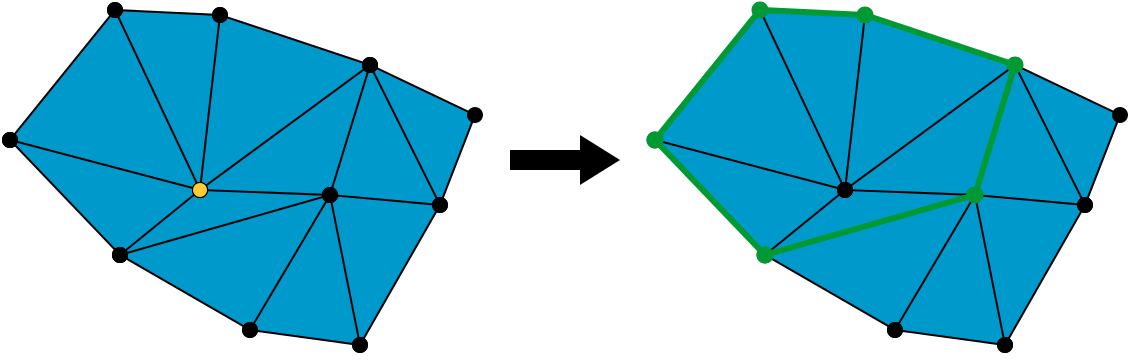
\includegraphics[width=.7\textwidth]{simplicial_complex_link.png}
    \caption[2D link]{2D三角网格上的link示意图,图引用自\cite{simplicial-complex}}
    \label{fig:link}
\end{figure}
从而边AB上的Link Condition定义为$Lk(A) \cap Lk(B) = LK(AB)$。从Link Condition中我们可以直观地发现,对于2D空间中的一个点A其Lk(A)为顶点A的一环邻域的边界上的顶点和边,而$Lk(AB)$则是包含边AB的三角形的另一个顶点,边AB的Link Condition是否满足等价于A和B各自一环邻域的边界不能相交于一条边,否则AB合并之后该边将成为一条孤立的边(不属于任何三角形,如图\ref{fig:2d-link-cond})。类似的对于3D空间上AB的Link Condition是否满足等价于A和B各自的一环邻域的边界不能相交于一个面,否则AB合并之后该面将成为一个孤立的面(不属于任何四面体,如图\ref{fig:3d-link-cond})。
\begin{figure}[htbp]
    \centering
    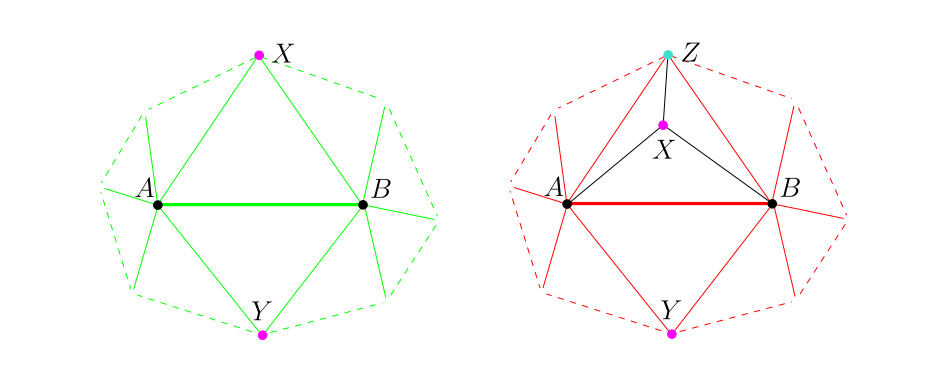
\includegraphics[width=.7\textwidth]{2d_link_cond.png}
    \caption[2D Link Condition]{2D三角网格上的Link Condition示意图,对于边AB,左图满足Link Condition,右图不满足Link Condition,图引用自\cite{isotopic-appro}}
    \label{fig:2d-link-cond}
\end{figure}
\begin{figure}[htbp]
    \centering
    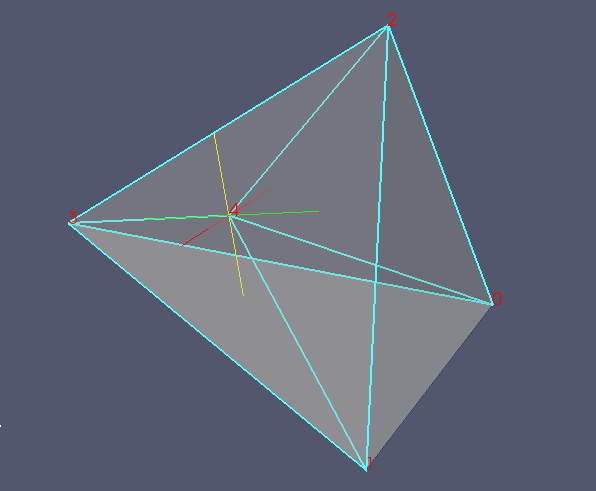
\includegraphics[width=.5\textwidth]{3d_link_cond.png}
    \caption[3D Link Condition]{3D三角网格上的Link Condition示意图,顶点1和3不能被合并,若顶点1和3合并,则会出现一个不属于任何四面体的三角面片024}
    \label{fig:3d-link-cond}
\end{figure}

\subsection{Kernel Region}
为了保证消边之后$\tau$仍然是包围球空间的一个有效填充,即不会产生四面体相互交叉的情况,需要保证得新生成的四面体是边PQ——环邻域的空间(由包含P或Q的四面体构成的空间)的有效填充。因此,PQ的合并点必须落在PQ的邻域空间的边界的每一个三角形内侧。我们定义该空间为边PQ的Kernel Region——$K_\tau(PQ)$(如图\ref{fig:kernel-region}是2D的Kernel Region示意图)。
\begin{figure}[htbp]
    \centering
    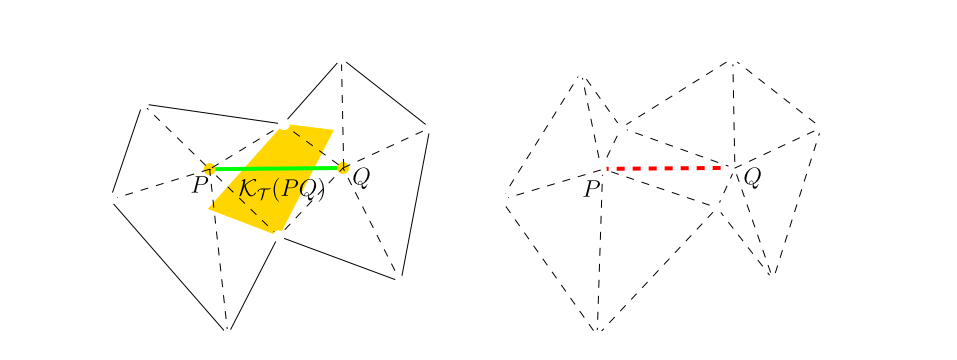
\includegraphics[width=.8\textwidth]{kernel_region.png}
    \caption[2D Kernel Region]{在二维中一条边的PQ的Kernel Region为PQ的一环邻域的三角面片边界上,每一条边所对应的直线的内侧(PQ这一侧)的交集,图引用自\cite{isotopic-appro}}
    \label{fig:kernel-region}
\end{figure}
\par 在对$\partial \Gamma$进行消边时,从内外壳的采样点中选取合并点。除了需要满足保持四面体网格$\tau$的有效性外,还需要保证满足误差控制条件$\forall s \in S, \delta(s) < 1$。因此,需要对$K_\tau (PQ) \cap S$中所有的点,逐个判断若合并到该点后,新生成的四面体空间中所有的采样点是否满足$\delta(s) < 1$,若满足则合并到这个点,否则继续尝试下一个点。若$K_\tau (PQ) \cup S$所有的点都无法保持$\delta(s) < 1$这个条件,则放弃消除这条边。和其他简化算法类似,为了找到一个更优的合并点的位置,使得误差更小,可以对所有的采样点根据其到PQ的2环邻域的每一个0-等值三角形所在平面的距离平方和由小到大做一个优先级排序。
\subsection{0-等值面的生成}
当误差边界$\partial \Gamma$简化完成之后,将$\tau$中每一条由连接内外边界$(\partial \Gamma_0, \partial \Gamma_1)$的边的中点——0-等值点嵌入到这个四面体中并细分这个四面体网格,从而得到由0-等值点构成的0-等值面$\mathcal{Ζ}$,现在$\mathcal{Z}$是在误差空间$\Omega$中原网格的一个同坯近似(如图\ref{fig:mutual-tessellation})。
\begin{figure}[htbp]
    \centering
    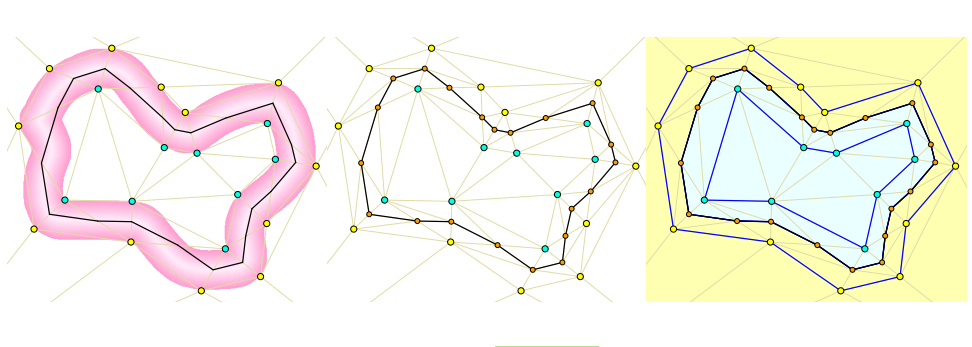
\includegraphics[width=.8\textwidth]{mutual_tessellation.png}
    \caption[Mutual tessellation]{在二维上的0-等值点嵌入:左图为在0-等值点嵌入之前;中间图为0-等值点嵌入之后;右图显示了$\partial \Gamma$的边界线蓝色线,以及0-等值线黑色线,以及函数$f(s)$的取值情况,黄色区域$f(s) > 0$,淡蓝色区域$f(s) < 1$,图引用自\cite{isotopic-appro}}
    \label{fig:mutual-tessellation}
\end{figure}

\subsection{所有可能的简化}
由于$\Gamma$是原误差空间$\Omega$的一个简化近似,因此,0-等值面的简化可能无法充分利用$\Omega$的空间(如图\ref{fig:tol-small})。为了尽可能充分地利用误差空间,可以通过尝试消除由0-等值点或边界上的点构成的边来调整0-等值点的位置,并扩大0-等值面上的边的Kernel Region,从而达到进一步简化的目的(如图\ref{fig:all-edges-collapse})。当所有简化都结束之后,最终的0-等值面就是我们的简化结果。

\begin{figure}[htbp]
    \centering
    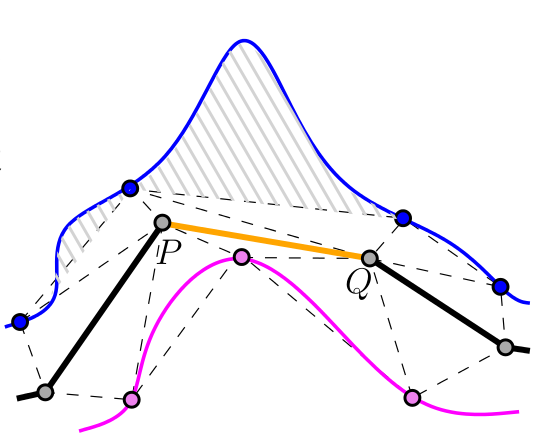
\includegraphics[width=.5\textwidth]{tol_small.png}
    \caption[无法利用的误差空间]{图中阴影部分空间无被充分利用起来,图引用自\cite{isotopic-appro}}
    \label{fig:tol-small}
\end{figure}

\begin{figure}[htbp]
    \centering
    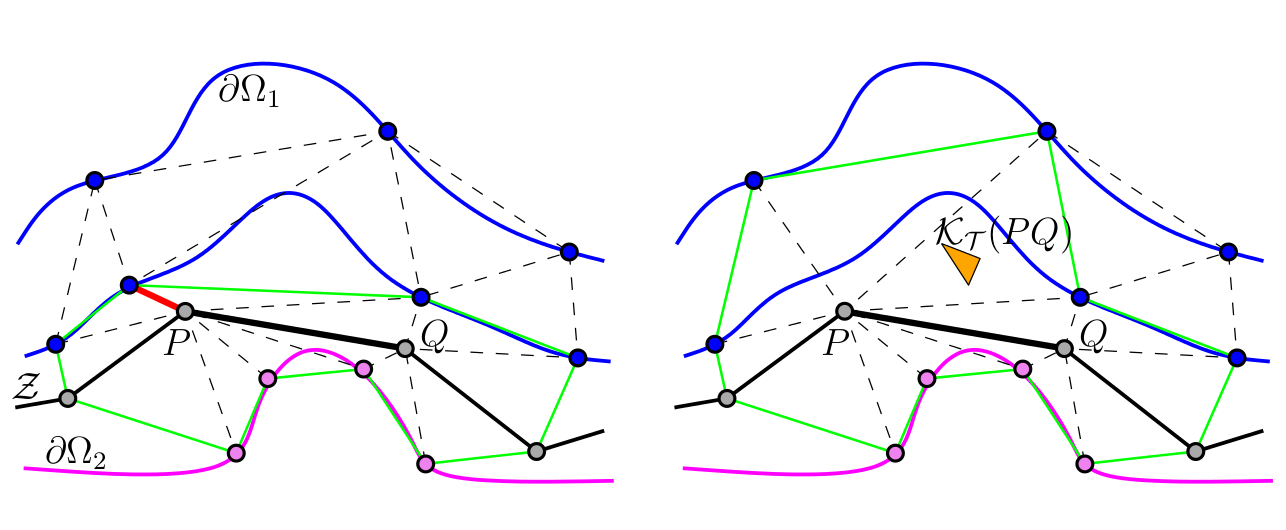
\includegraphics[width=.9\textwidth]{zb_collapse.png}
    \caption[所有可能的边的消除]{通过消除所有可能的边来进一步简化网格。左图中边PQ由于Kernel Region为空而无法消除,在右图中通过消除左图中的红色边,PQ的Kernel Region变为橙色的区域(不为空),从而增大了PQ消除的可能性。图引用自\cite{isotopic-appro}}
    \label{fig:all-edges-collapse}
\end{figure}

\section{本章小结}
本章详细介绍了Manish Mandad等人提出的网格同坯近似算法\cite{isotopic-appro}。本章首先简述了该算法的其特点,并详细介绍了其主要步骤。该算法以误差空间$\Omega$的边界上的采样点S作为输入。以S的包围球上的顶点初始化顶点,利用 3D Delaunay三角化建立起一个四面体网格$\tau$,并在这个四面体网格上维护一个误差函数$\epsilon(s)$,贪心地从S中选取误差最大的顶点插入到$\tau$中,直到S中所有点的误差不超过1。然后在保持$\tau$有效、保持误差约束和保持法向约束条件的前提下、通过简化误差边界,得到一个更加稀疏的误差空间$\Omega$的近似。再通过嵌入0-等值点得到显示的0-等值面。最后通过简化0-等值面和所有可能的简化得到最终的简化结果。
%% 通过阅读上一章节,
%% 相信您已基本配置好了自己的编辑环境,
%% 了解了如何正确编写各级章节、段落和子段落,
%% 容易引起编译出错的逃逸字符。

%% 从上一章出现过的有序列表、外部图片和代码环境中,
%% 您应该已经发现,
%% 使用命令\texttt{$\backslash$begin\{xxxx\}}可以开始一段新的布局环境。
%% 这一章将系统地阐述计算机类的学位论文需要排版的元素的编写方法。
%% 主要包括以下排版要素:
%% \begin{itemize}
%%     \item 列表环境(包括有序、无序、定义三种列表)
%%     \item 插图和表格
%%     \item 代码环境
%%     \item 数学和算法环境
%% \end{itemize}

%% 这一章只涉及为完成此排版环境的宏包的最基本使用方法,
%% 本章尽量覆盖论文写作中的大部分场景,
%% 如有特殊需求,请仔细阅读相关宏包手册并求助于国内外TeX社区及问答网站。

%% \section{列表环境}

%% 列表环境有三种,
%% 类似与HTML的\texttt{<ol>},
%% \texttt{<ul>},\texttt{<dl>}
%% 三个标签。
%% 以下是一个定义列表环境:
%% \begin{description}
%%     \item[有序列表] enumerate 默认从阿拉伯数字1开始编号,如需更改请搜“重定义列表”
%%     \item[无序列表] itemize 默认圆点标记,尽量少用此类列表
%%     \item[定义列表] description 语义上用于作一系列简短的解释
%% \end{description}

%% 列表可以嵌套,比如:
%% \begin{enumerate}
%% 	\item 第一级列表
%% 	\item 第一级列表
%% 	\begin{enumerate}
%% 		\item 第二级列表
%% 		\item 第二级列表
%%         \begin{itemize}
%%             \item 第三级列表
%%             \item 第三级列表
%% 		\end{itemize}
%% 		\item 第二级列表
%% 		\item 第二级列表
%% 	\end{enumerate}
%% \end{enumerate}

%% \section{插图环境和浮动体}

%% 相信您在上一章的探索学习中已经基本掌握了如何插入图片的方法,
%% 但可能仍存疑虑。
%% 所以现在先简单介绍浮动体的概念以助您理解插图环境的布局规则,
%% 最后再介绍子图的排布以应对您更高的布局需求。
%% % 关于绘图,本文将在后续章节讲述
%% % 活用引用,让评阅老师随处移动
%% 关于图的绘制,本文将在\ref{how-to-plot} 继续讲述。

%% 当一个图片或表格太大在当前页面无法继续排布时,
%% 一种解决方案就是新开一页再排布(Word 默认使用此种)。
%% 这个方法在页面上留下分空白,十分不美观。
%% \LaTeX 的默认解决方案是把它们“浮动”到下一页,
%% 与此同时使用后续正文文本填充当前的空白。

%% 插图和表格在\LaTeX 排版中被默认当成浮动体对待,
%% 当排版引擎试图放置一个浮动体时,它将遵循以下规则:
%% \begin{enumerate}
%%     \item 浮动体的布局大小不得超过版心的大小,否则抛出Overfull Page错误
%%     \item 浮动体只会向后浮动,不会向前浮动
%%     \item 浮动体默认按照 h $\to$ t $\to$ b $\to$ p 的规则布局
%%     \begin{description}
%%         \item[h] 当前位置,如果本页所剩空间不够,这一参数无效
%%         \item[t] 浮动到下一页顶部
%%         \item[b] 浮动到下一页底部(脚注之下)
%%         \item[p] 浮动到一个允许出现浮动体的页面上
%%         \item[!] 忽略浮动体放置的大多数内部参数\footnote{作者也不太懂}
%%     \end{description}
%%     \item 设置 htbp 参数的顺序不会影响默认的规则顺序
%% \end{enumerate}

%% 在实践中,一般选用浮动规则[htbp], [tbp], [htp], [tp] 来完成浮动体布局。
%% 请不要使用单一参数布局,这样极有可能出现难解的浮动问题。
%% 不适当的浮动规则参数将导致浮动对象被放进一个队列中等待布局,
%% 这个队列的默认大小是18,如果队列超限,编译中会抛出一个Too Many Unprocessed Floats错误。
%% 如果一页图片太多,甚至几乎占满一个版心,
%% 您可以通过\texttt{$\backslash$clearpage}命令强制在此处必须排版完所有浮动体
%% 再排版之后内容,关于清除浮动等复杂主题,这里不再展开。
%% 此处只能建议插图尺寸不宜过大,插图密度不宜过大。
%% 考虑到图文混排的最佳视觉要求,
%% 可以待论文内容稳定下之后,仔细调整插图代码的位置,
%% 通过前置插图代码,强行“向后浮动”,保证插图和引用处足够近。

%% 关于模板对浮动体的设置,参看\texttt{zjuthesis.cls},
%% 搜索关键字“浮动体”找到对应配置。
%% 图片引用路径在\texttt{zjuthesis.cls}里定义的\texttt{graphicspath}里,
%% 默认情况下\\\texttt{$\backslash$includegraphics}命令从论文源码根目录搜索引用的图片,
%% 如果先在根目录里匹配到文件名,则不再前往定义路径搜索,
%% 当引擎无法找到您指定的图片资源时,会导致编译错误。
%% 注意引用的文件名包括文件后缀。

%% % 现在你可以随意更动此插图代码的位置来感受一下浮动体布局的规则
%% \begin{figure}[htbp]
%% 	\centering
%% 	\begin{subfigure}[b]{.45\textwidth}  % 注意此处的尺寸控制
%% 		\centering
%% 		\includegraphics[width = \textwidth]{xuejian.jpg}
%% 		\caption{仙三}\label{fig:subfig-samp1}
%% 	\end{subfigure}
%% 	\begin{subfigure}[b]{.45\textwidth}
%% 		\centering
%% 		\includegraphics[width = \textwidth]{wenhui.jpg}
%% 		\caption{仙三外}\label{fig:subfig-samp2}
%% 	\end{subfigure}
%% 	\begin{subfigure}[b]{.45\textwidth}
%% 		\centering
%% 		\includegraphics[width = \textwidth]{lingsha.jpg}
%% 		\caption{仙四}\label{fig:subfig-samp3}
%% 	\end{subfigure}
%% 	\caption{仙剑白学传}\label{fig:subfig-samp}
%% \end{figure}

%% 接下来描述一下子图的编写,
%% 在实际论文撰写过程中,
%% 经常遇到需要比较几组实验数据或场景的需求。
%% 此时,合乎语义的做法是为不同的组设置子图,
%% 而不是分别设图。

%% 多个子图组成一个单独的浮动体进行布局,
%% 共用一个总图题总引用,并可以有各自单独的子图题和交叉引用。
%% 本模板使用subcaption 宏包处理子图排版问题,如\autoref{fig:subfig-samp} 所示
%% \footnote{不要在正式论文排版过程中使用彩色区分类别,论文最终以灰度打印}。
%% 论文中不可像本文一般,
%% 平白无故地出现与行文毫无关联的图例,
%% 而且,必须有适当的文字内容对图例做出解释。
%% 比如比较分析从\autoref{fig:subfig-samp1} 到\autoref{fig:subfig-samp3}
%% 仙剑系列在白学梗方面的运用变迁。\footnote{往后数代仍有类似场景 -\_-\# (顔文字書込禁止!)}

%% 当准备插图资源时,应该尽可能保证插图清晰,背景透明。
%% 图中文字大小与文中接近,不小于脚注大小,不大于正文段落文字大小,
%% 框线宽度不大于2px。

%% 如果您曾关注过图片格式,
%% 应该知道图片在计算机中一般分为矢量图(\autoref{fig:vector})和位图(\autoref{fig:raster})两种类型。
%% 通俗地理解,矢量图通过几何属性存储信息,所以在缩放时保持图形的几何属性。
%% 而位图按像素点存储信息,在缩放时必然丢失信息。
%% 对于学位论文里的大部分为表达实验数据而描述的图例,最好使用矢量图绘制,
%% 以给评阅老师或后人精确地参考和还原实验。
%% 常用的矢量图格式有eps, pdf, svg 和 Adobe 系列的文件格式。
%% 其中\LaTeX 格式可以直接引用eps 和 pdf 格式的图片。

%% \begin{figure}[htbp]
%% 	\centering
%% 	\begin{subfigure}[b]{.45\textwidth}
%% 		\centering
%% 		\includegraphics[width = \textwidth]{vector.pdf}
%% 		\caption{矢量图}\label{fig:vector}
%% 	\end{subfigure}
%% 	\begin{subfigure}[b]{.45\textwidth}
%% 		\centering
%% 		\includegraphics[width = \textwidth]{raster.png}
%% 		\caption{位图}\label{fig:raster}
%% 	\end{subfigure}
%% 	\caption{Google Logo 的矢量图和位图比较}\label{fig:vector-raster}
%% \end{figure}


%% \section{表格}
%% 表格与插图一样,也是浮动体。
%% 在\LaTeX 中,表格的编写成本比较高,
%% 极易引发编译错误。
%% 对于只有两列的表格,建议改用列表环境完成排版。
%% 本模板使用tabu环境排版表格,
%% 使用longtabu环境排版超长表格。
%% 学术论文多用线条简洁的三线表,
%% 所谓三线就是 toprule, midrule和bottomrule 。
%% 如\autoref{tab:tabu_test_1} 是对tabu宏包的tabu表格环境测试。
%% \begin{table}[htbp]
%% 	\centering
%% 	\caption{这是一个用tabu环境的测试用的表格}\label{tab:tabu_test_1}
%%     \begin{tabu}{lrr} % lrr 表示 左对齐 右对齐 右对齐
%%     %\begin{tabu}{|l|r|r|} % 加上竖线看看

%%     \toprule % 软件学院论文模板规定表头必须加粗
%%     \textbf{行星}     & \textbf{赤道半径}km & \textbf{公转周期}d \\
%%     \midrule
%%     水星     & 2.439  & 87.9 \\
%%     金星     & 6.1    & 224.682 \\
%%     地球     & 6378.14 & 365.24 \\
%%     \bottomrule
%%     \end{tabu}%
%% \end{table}

%% \autoref{tab:tabu_test_2} 对tabu to表格的x列模式进行测试。在表格导言区中设置为X[1]X[2]X[2],表示这三列表格的列宽比值为1:2:2,总的表格宽度由tabu to环境设置,这里设置为0.6\textbackslash linewidth。相比于tabular环境,tabu环境的列宽设置方便许多。
%% \begin{table}[htbp]
%% 	\centering
%% 	\caption{tabu环境测试表格---X列模式}\label{tab:tabu_test_2}
%%     \begin{tabu} to 0.6\linewidth{X[1]X[2]X[2]}
%%     \toprule
%%     \textbf{行星}     & \textbf{赤道半径}km & \textbf{公转周期}d \\  % 为了表格排版的美观 表头建议加粗
%%     \midrule
%%     水星     & 2.439  & 87.9 \\
%%     金星     & 6.1    & 224.682 \\
%%     地球     & 6378.14 & 365.24 \\
%%     \bottomrule
%%     \end{tabu}%
%% \end{table}

%% 如\autoref{tab:tabu_test_3}是longtabu环境测试表格。
%% longtabu环境不能用在table浮动体环境中。
%% 根据GB/T 7713.1-2006规定:如果某个表需要转页接排,
%% 在随后的各页上应重复表的编号。
%% 编号后跟标题(可省略)和“(续)”, % 表:「我要续…… +1
%% 置于表上方。
%% 续表应重复表头。

%% 特别需要注意的是,
%% longtabu是基于longtable宏包开发的,
%% 所以在zjuthesis.cls文件中已经插入了longtable宏包。
%% longtable环境的所有功能都可以在longtabu中使用,
%% 如\textbackslash endhead,
%% \textbackslash endfirsthead,
%% \textbackslash endfoot,
%% \textbackslash endlastfoot,
%% 和\textbackslash caption等。
%% 具体用法请参见longtable和tabu宏包的相应文档。

%% \begin{longtabu}{lccc}
%% \caption{材料弹性模量及泊松比}\label{tab:tabu_test_3}\\
%% \toprule
%% 名  称   & 弹性模量E/Gpa & 切变模量G/Gpa & 泊松比$\mu$ \\
%% \midrule%
%% \endfirsthead
%% \caption{材料弹性模量及泊松比(续)}\\
%% \toprule
%% 名  称   & 弹性模量E/Gpa & 切变模量G/Gpa & 泊松比$\mu$ \\
%% \midrule%
%% \endhead
%% \bottomrule%
%% \endfoot
%% 镍铬钢、合金钢 & 206    & 79.38  & 0.3 \\
%% 碳 钢    &  196~206 & 79     & 0.3 \\
%% 铸 钢    &  172~202 &        & 0.3 \\
%% 球墨铸铁   &  140~154 &  73~76 & 0.3 \\
%% 灰铸铁、白口铸铁 &  113~157 & 44     &  0.23~0.27 \\
%% 冷拔纯铜   & 127    & 48     &   \\
%% 轧制磷青铜  & 113    & 41     &  0.32~0.35 \\
%% 轧制纯铜   & 108    & 39     &  0.31~0.34 \\
%% 轧制锰青铜  & 108    & 39     & 0.35 \\
%% 铸铝青铜   & 103    & 41     & 0.3 \\
%% 冷拔黄铜   &  89~97 &  34~36 &  0.32~0.42 \\
%% 轧制锌    & 82     & 31     & 0.27 \\
%% 硬铝合金   & 70     & 26     & 0.3 \\
%% 轧制铝    & 68     &  25~26 &  0.32~0.36 \\
%% 铅      & 17     & 7      & 0.42 \\
%% 玻璃     & 55     & 22     & 0.25 \\
%% 混凝土    &  14~39 &  439~15.7 &  0.1~0.18 \\
%% 纵纹木材   &  9.8~12 & 0.5    &   \\
%% 横纹木材   &  0.5~0.98 &  0.44~0.64 &   \\
%% 橡胶     & 0.00784 &        & 0.47 \\
%% 电木     &  1.96~2.94 &  0.69~2.06 &  0.35~0.38 \\
%% 赛璐珞    &  1.71~1.89 &  0.69~0.98 & 0.4 \\
%% 可锻铸铁   & 152    &        &  \\
%% 拔制铝线   & 69     &        &  \\
%% 大理石    & 55     &        &  \\
%% 花岗石    & 48     &        &  \\
%% 石灰石    & 41     &        &  \\
%% 尼龙1010 & 1.07   &        &  \\
%% 夹布酚醛塑料 &  4~8.8 &        &  \\
%% 石棉酚醛塑料 & 1.3    &        &  \\
%% 高压聚乙烯  &  0.15~0.25 &        &  \\
%% 低压聚乙烯  &  0.49~0.78 &        &  \\
%% 聚丙烯    &  1.32~1.42 &        &  \\
%% 硬聚氯乙烯  &  3.14~3.92 &        &  \\
%% 聚四氟乙烯  &  1.14~1.42 &        &  \\
%% \end{longtabu}%


%% \section{代码段}

%% 原则上,论文中应尽量少的出现代码段。
%% 如果不得不引用一小部分代码,
%% 可以使用\texttt{lstlisting}设置代码环境。
%% 本模板的代码环境默认配置在\texttt{zjuthesis.cls}搜索关键字“代码”。

%% 因本模板不鼓励引用大段代码,
%% 所以默认情况下不为代码开启行号。
%% 观查\autoref{code:samp-code},结合前述图表设置,
%% 试图理解代码环境的编写。

%% \begin{lstlisting}[language=C++,numbers=left, numberstyle=\tiny,label=code:samp-code, caption=一段Chromium的源代码]
%% // Start tasks to take all the threads and block them.
%%   const int kNumBlockTasks = static_cast<int>(kNumWorkerThreads);
%%   for (int i = 0; i < kNumBlockTasks; ++i) {
%%     EXPECT_TRUE(pool()->PostWorkerTask(
%%         FROM_HERE,
%%         base::Bind(&TestTracker::BlockTask, tracker(), i, &blocker)));
%%   }
%%   tracker()->WaitUntilTasksBlocked(kNumWorkerThreads);

%%   // Setup to open the floodgates from within Shutdown().
%%   SetWillWaitForShutdownCallback(
%%       base::Bind(&TestTracker::PostBlockingTaskThenUnblockThreads,
%%                  scoped_refptr<TestTracker>(tracker()), pool(), &blocker,
%%                  kNumWorkerThreads));
%%   pool()->Shutdown(kNumWorkerThreads + 1);

%%   // Ensure that the correct number of tasks actually got run.
%%   tracker()->WaitUntilTasksComplete(static_cast<size_t>(kNumWorkerThreads + 1));
%%   tracker()->ClearCompleteSequence();
%% \end{lstlisting}

%% 引用一两行代码,可以直接使用\texttt{verbatim}环境完成。
%% 注意此环境不会采取任何主动断行策略。
%% \begin{verbatim}
%% Error: Command failed: /bin/sh -c rsync -arvq --exclude cache
%% --exclude .git 
%% \end{verbatim}

%% \section{数学和算法环境}

%% \TeX 模板引擎创立之初就是为了最美观地排版本节的主题。
%% 在理工科的学位论文中,数学符号和数学公式必不可少
%% \footnote{至于定理、引理和推论等纯理科环境,本模板未作任何设定,不讨论。}。
%% 在本模板中,数学环境由amsmath和amssymb宏包支持。
%% 即便没有使用公式,您应该也希望看到$a_1$, $a_2$, $a_3$而不是a1, a2, a3 吧?

%% 于简单的行内公式,
%% 直接在源码处编写\texttt{\$...\$}内的公式即可,
%% 不熟习\LaTeX 公式编写的同学,
%% 可以使用可视化的公式编辑器产生\LaTeX 代码,
%% 这里推荐使用Daum Equation Editor完成复杂公式编辑的工作。

%% 对于单行公式,可以使用\texttt{\$\$...\$\$}创建。
%% $$Y=\sum_{k=1}^n X_k$$
%% 如果需要设定交叉引用,那推荐align环境创建,如\eqref{eq:samp}所示。
%% \begin{align}\label{eq:samp}
%%     f(x) & = 2(x + 1)^{2} - 1\\                  % & 用来对齐等号
%% 		 & = 2(x^{2} + 2x +1)-1\\
%% 		 & = 2x^{2} + 4x + 1
%% \end{align}

%% %一个矩阵
%% %$$\begin{bmatrix}
%% %1&2&3&4\\
%% %5&6&7&8\\
%% %9&10&11&12
%% %\end{bmatrix}$$

%% 计算机类的学位论文
%% 一般少不了对研究算法的描述。
%% 本模板选用algorithmi2e宏包排版算法环境。
%% 详细指令使用方式参见宏包使用手册
%% \footnote{一般有需求排布复杂算法的同学应该有一定的科研经历}。
%% 如\autoref{algo:duplicate2}

%% \begin{algorithm}
%% \DontPrintSemicolon
%% \KwIn{A sequence of integers $\langle a_1, a_2, \ldots, a_n \rangle$}
%% \KwOut{The index of first location with the same value as in a previous location in the sequence}
%% $location \gets 0$\;
%% $i \gets 2$\;
%% \While{$i \leq n \land location = 0$} {
%%   $j \gets 1$\;
%%   \While{$j < i \land location = 0$} {
%%     % The "l" before the If makes it so it does not expand to a second line
%%     \lIf{$a_i = a_j$} {
%%       $location \gets i$\;
%%     }
%%     \lElse{
%%       $j \gets j + 1$\;
%%     }
%%   }
%%   $i \gets i + 1$\;
%% }
%% \Return{location}\;
%% \caption{{\sc FindDuplicate2}}
%% \label{algo:duplicate2}
%% \end{algorithm}

%% \section{绘图}\label{how-to-plot}

%% 一图胜千言,经过同学们辛苦的实验积累下的数据,
%% 应该尽量以最高质量呈现出来,而不是使用冗长的语句反复言说。
%% 使用强大的TikZ宏包,可以绘制各式各样的图例,
%% 比如在\ref{dirtree} 的目录结构图就是使用TikZ宏包绘制完成。
%% 通过绘图宏包得到的是矢量图,
%% 经过缩放后仍能精确地指导打印。
%% 由于使用TikZ宏包绘制各式图例的方法艰深繁杂,
%% 非长期钻研学术者实不可速取。

%% % 这里删掉了一大段TikZ宏包的使用
%% % 太复杂了  如果不是跟老师搞学术的话真的算了

%% 含有大量数据的统计图,
%% 从事数据分析工作的同学可自行使用python或R语言完成绘制,
%% 确保输出eps或pdf格式图形,使用插图环境引入即可。

%% 对于一般的流程图,本模板推荐使用graphviz绘图工具绘制。
%% 相对于TikZ,graphviz已经足够适合人类掌握了。
%% 如果坚持使用可视化工具完成此类图例的绘制,
%% 本文推荐一个在线绘图工具\texttt{https://www.draw.io},
%% 该工具可以绘制流程图、UML系列和很多可以引入的小图标。
%% 另外它还支持dropbox同步及输出pdf,通过同步论文的图片引用目录,
%% 可以最高效的完成绘图和插图的工作。

%% 无论用何种工具完成绘图,
%% 时间精力成本都不会太低。
%% 请妥善规划您的论文撰写时间,
%% 确保顺利毕业。

%% \section{关于参考文献}

%% 硕士学位论文的参考文献学院规定至少20篇以上,
%% 不可滥引,注重引文质量。

%% 参考文献标准参照国家标准《GB/T 7714-2005: 文后参考文献著录规则》\footnote{此标准规定的学位论文引用格式并无指定需列出是“硕士学位论文”还是“博士学位论文”}。
%% 样式文件由南京大学胡海星提供。
%% \begin{verbatim}
%% http://haixing-hu.github.io/nju-thesis/
%% \end{verbatim}

%% 参考文献采用顺序编码制,即引文处采用序号标注,参考文献表按引文序号列出。
%% 参考文献的排版需要引入同学们自己的参考文献数据库,
%% 南京大学胡海星提供了一个样例数据库,见\texttt{references/test.bib}。
%% 建议通过各式文献管理工具,在论文早期工作时逐渐积累文献数据库。
%% 通过Google学术查找一篇文献时,如\autoref{fig:gscholar} 所示,点击cite,
%% 选择BibTeX,即可得到本文献的Bib格式的各项字段。
%% \begin{figure}[htbp]
%%     \centering
%%     \includegraphics[width=\textwidth]{gscholar.png}
%%     \caption{使用Google学术查找引文的BibTeX字段}
%%     \label{fig:gscholar}
%% \end{figure}

%% 注意,由Google学术提供的文献类型和字段有可能不满足胡海星的设定,
%% 注意调整。
%% 胡海星提供的参考文献样式表中设定的文献类型列出:
%% \begin{description}
%%     \item[期刊]          \texttt{@article}
%%     \item[专著]          \texttt{@book, @inbook}
%%     \item[译著]          \texttt{@Book, @inBook}
%%     \item[会议论文集]    \texttt{@proceeding, @inproceeding}
%%     \item[手册]          \texttt{@manual}
%%     \item[网页]          \texttt{@webpage, @online}
%% \end{description}

%% \begin{itemize}
%%     \item 比如这是一篇中文期刊\cite{lixiaodong1999}
%%     \item 这是几篇英文期刊\cite{christine1998, kanamori1998}
%%     \item 一本中文书\cite{zh-book-1}
%%     \item 一本中文译著\cite{anwen1988b}
%%     \item 一本英文书\cite{lamport1994latex, takeuti1973}
%%     \item 一篇中文inproceeding\cite{nonlinear1996}
%%     \item 中文proceeding\cite{a2-1}
%%     \item 英文proceeding\cite{a2-2}
%%     \item 中文inproceeding\cite{aczel1998}
%%     \item 一篇学位论文\cite{a4-1} 
%%     \item 其他资料:手册\cite{ipad}报纸\cite{renminribao}网页\cite{dubash2010}
%% \end{itemize}

%% 在论文中设置了一个错误或丢失的引用不会引起编译错误,
%% 引擎会在引用标记中设一个问号。
%% 手动编译论文的顺序一般为:
%% \begin{verbatim}
%% xelatex main
%% bibtex main  // 生成参考文献
%% xelatex main
%% xelatex main
%% \end{verbatim}
%% latexmk 自动化地执行了这些步骤,所以编译时间才需要20余秒之久。

%% \section{本章小结}

%% 本章划分节比较多,正式行文中请尽量避免。

%% 传播智识,单单借助文字的力量是相对无力的,
%% 即使是日常博文,列表、插图、表格、代码都少不了。
%% 何况是一篇用于申请硕士学位的论文呢?

%% 一篇学位论文集长期的科研工程实践智慧于寥寥数万字。
%% 如何合理规划论文语义和排版元素,
%% 让即便不熟习此领域的后人能在短时间内消化,
%% 继续开物前民,
%% 是同学们应该在论文撰写过程中反复求索的。


